

\subsection*{Ход работы (шум фактор и темновой счёт)}



\textbf{Частота темнового счёта SiPM}.
Перейдем в режим регистрации экстремумов (рис. 2), и установим временное разрешение в 80 ns. Измерим частоты темнового счёта с различным разрешением res (см. таблицу 1). 


 Построим зависимость (см. рис. \ref{fig:1}) частоты темнового счёта $f$ от разрешения peak-detect,
где $f$ можем найти, как
\begin{equation*}
    f = \frac{\text{hits}}{\text{wfms} \times T},
\end{equation*}
где wfms -- количество разверток, hits -- количество зарегистрированных импульсов, $T$ -- время развертки осциллографа, равно $0.1$ ms.

\begin{figure}[h]
    \centering
    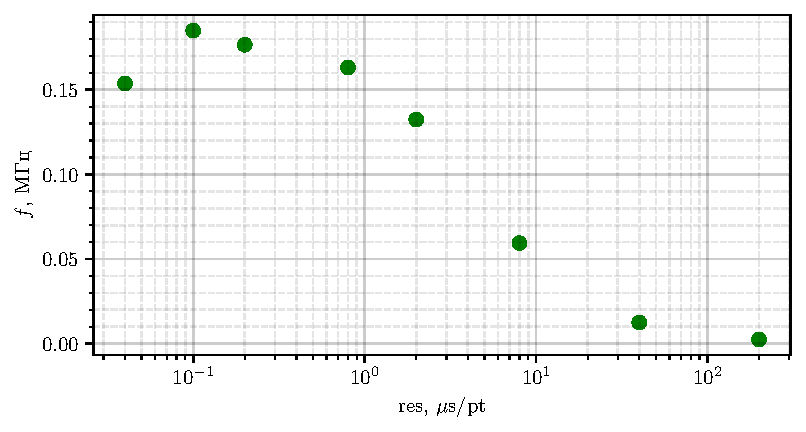
\includegraphics[width=0.75\textwidth]{figures/plot1.pdf}
    \vspace{-5mm}
    \caption{Зависимость частоты темнового счёта $f$ от разрешения res}
    \label{fig:1}
\end{figure}

Можно явно разделить зависомость $f(\text{res})$ на две области, разграниченные значением в $1 \ \mu$с. Чем меньше res, тем чаще импульсы попадают на границу дух временных интервалов, от чего эффектиное значение $f$ увеличивается. Чем больше res, тем чаще неcколько импульсов попадает в один интервадл, от чего эффективное значение $f$ уменьшается. 

Таким образом res $ = 1 \ \mu$с находится в промежутке между длительностью одного импульса и средним периодом повторения, а значит искомое значение частота темнового счёта:
\begin{equation*}
    f = (0.17 \pm 0.02) \text{ МГц}.
\end{equation*}


\textbf{Шум фактор SiPM}. 
Для расчета шум-фактора воспользуемся формулой
$$
F = 1 + \frac{\sigma^2}{\mu^2} = 1.026,
$$
где параметры взяты из гистограммы для разрешения 200\,нс. Из $\sigma$ дополничтельно вычтена $\sigma_\text{sys}$.




\textbf{Оценка величины заряда}
Оценить можно тремя способами.
Во-первых, зная темновой ток и частоту темнового счета $f$ имеем:
$$
q = \frac{I_\text{dark}}{f} = (3.1\pm 0.4)\times 10^{-14}\,\text{Кл} = (1.9\pm 0.2)\times  10^5\, e,
$$
где $e$ -- заряд электрона. 
Во-вторых, исходя из формы пика (рис. \ref{fig:0}) и внутреннего сопротивления осциллографа $R=50\,\text{Ом}$:
$$
q = \frac{1}{R}\int\limits_\text{pike} U(t) \d t \approx \frac{1}{R} \times \text{high} \times  \text{width} = 
\frac{1}{50 \ \Omega} \times  (20 \, \text{мВ})\times (2\, \text{ns}) \approx  5 \times  10^6 e.
$$
В третьих, из прошлой работы известно, что по порядку величины емкость фотодетектора $C \approx 20\,\text{пФ}$, откуда:
$$
q \approx C \cdot \mu = 5\cdot 10^{-13}\,\text{Кл} = 3 \cdot 10^6\, e.
$$
Стандартные отклонения могут быть получены из отклонения амплитуды импульсов:
$$
\frac{\sigma_q}{q} = \frac{\sigma}{\mu} = 0.16.
$$